% $Header: /Users/joseph/Documents/LaTeX/beamer/solutions/conference-talks/conference-ornate-20min.en.tex,v 90e850259b8b 2007/01/28 20:48:30 tantau $

\documentclass{beamer}

% This file is a solution template for:

% - Talk at a conference/colloquium.
% - Talk length is about 20min.
% - Style is ornate.



% Copyright 2004 by Till Tantau <tantau@users.sourceforge.net>.
%
% In principle, this file can be redistributed and/or modified under
% the terms of the GNU Public License, version 2.
%
% However, this file is supposed to be a template to be modified
% for your own needs. For this reason, if you use this file as a
% template and not specifically distribute it as part of a another
% package/program, I grant the extra permission to freely copy and
% modify this file as you see fit and even to delete this copyright
% notice. 


\mode<presentation>
{
  \usetheme{Frankfurt}
  % or ...

  \setbeamercovered{transparent}
  % or whatever (possibly just delete it)
}


\usepackage[brazilian]{babel}
% or whatever


\usepackage{lmodern}			% Usa a fonte Latin Modern			
\usepackage[T1]{fontenc}		% Selecao de codigos de fonte.
\usepackage[utf8]{inputenc}		% Codificacao do documento (conversão automática dos acentos)
\usepackage{indentfirst}		% Indenta o primeiro parágrafo de cada seção.
\usepackage{color}				% Controle das cores
\usepackage{graphicx}			% Inclusão de gráficos
\usepackage{microtype} 			% para melhorias de justificação
\usepackage{eurosym}			% habilita símbolo do Euro
% Or whatever. Note that the encoding and the font should match. If T1
% does not look nice, try deleting the line with the fontenc.


\title[Rede PROFIBUS] % (optional, use only with long paper titles)
{Rede PROFIBUS}

\subtitle
{Seminário de Instrumentação e Automação}

\author[Arnaldo Viana, Otávio Petito, Tiago Demay] % (optional, use only with lots of authors)
{Arnaldo Viana\inst{1} \and Otávio Petito\inst{2} \and Tiago Demay\inst{3}}
% - Give the names in the same order as the appear in the paper.
% - Use the \inst{?} command only if the authors have different
%   affiliation.

\institute[Escola de Engenharia Mauá] % (optional, but mostly needed)
{
  \inst{1}%
  RA 09.01746-0\\
  6º Ano - Noturno
  \and
  \inst{2}%
  RA 08.1453-0\\
  6º Ano - Noturno
  \and
  \inst{3}%
  RA 09.02270-8\\
  6º Ano - Noturno
  }
% - Use the \inst command only if there are several affiliations.
% - Keep it simple, no one is interested in your street address.

\date[SCS 2015] % (optional, should be abbreviation of conference name)
{São Caetano do Sul, 2015}
% - Either use conference name or its abbreviation.
% - Not really informative to the audience, more for people (including
%   yourself) who are reading the slides online

\subject{Engenharia Elétrica - Ênfase Eletrônica}
% This is only inserted into the PDF information catalog. Can be left
% out. 



% If you have a file called "university-logo-filename.xxx", where xxx
% is a graphic format that can be processed by latex or pdflatex,
% resp., then you can add a logo as follows:

\pgfdeclareimage[height=0.5cm]{university-logo}{./figs/maua_logo}
\logo{\pgfuseimage{university-logo}}



% Delete this, if you do not want the table of contents to pop up at
% the beginning of each subsection:
%\AtBeginSubsection[]
%{
%  \begin{frame}<beamer>{\textit{Outline}}
%    \tableofcontents[currentsection,currentsubsection]
%  \end{frame}
%}


% If you wish to uncover everything in a step-wise fashion, uncomment
% the following command: 

\beamerdefaultoverlayspecification{<+->}


\begin{document}

\begin{frame}
  \titlepage
\end{frame}

\begin{frame}{\textit{Overview}}
  \tableofcontents
  % You might wish to add the option [pausesections]
\end{frame}


% Structuring a talk is a difficult task and the following structure
% may not be suitable. Here are some rules that apply for this
% solution: 

% - Exactly two or three sections (other than the summary).
% - At *most* three subsections per section.
% - Talk about 30s to 2min per frame. So there should be between about
%   15 and 30 frames, all told.

% - A conference audience is likely to know very little of what you
%   are going to talk about. So *simplify*!
% - In a 20min talk, getting the main ideas across is hard
%   enough. Leave out details, even if it means being less precise than
%   you think necessary.
% - If you omit details that are vital to the proof/implementation,
%   just say so once. Everybody will be happy with that.

\section{O que é?}

\subsection{Rede PROFIBUS}

\begin{frame}{PROFIBUS}{Protocolo de comunicação}
  % - A title should summarize the slide in an understandable fashion
  %   for anyone how does not follow everything on the slide itself.

  É um dos protocolos de comunicação que fazem parte do grupo dos \textit{fieldbuses} abertos e independentes de fornecedores, que permitem a integração de equipamentos de diversos fabricantes em uma mesma rede.
  
  \begin{figure}
  	\centering
  	
\includegraphics[scale=0.8]{figs/profibus.png} 
  \end{figure}
  
\end{frame}

\subsection{Histórico}

\begin{frame}{Histórico}{Alemanha, 1987}

	\begin{itemize}
		\item 1987 - PROFIBUS FMS (\textit{Fieldbus Message Specification});
		\item 1993 - PROFIBUS DP (\textit{Decentralized Periphery});
		\item 1995 - PROFIBUS PA (\textit{Process Automation}).
		
	\end{itemize}
 
\end{frame}


\section{PROFIBUS DP}

\subsection{Modelo OSI}

\begin{frame}{Modelo OSI}

	\begin{figure}
	\centering
	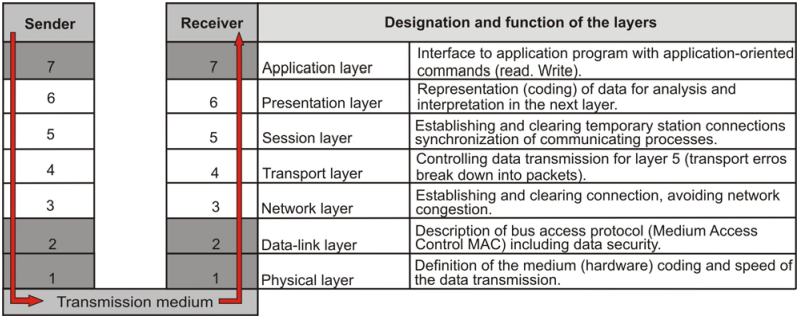
\includegraphics[scale=0.4]{figs/osi}
	\end{figure}

\end{frame}

\subsection{Características}

\begin{frame}{Características}{PROFIBUS DP}
	
	\begin{figure}
	\centering
	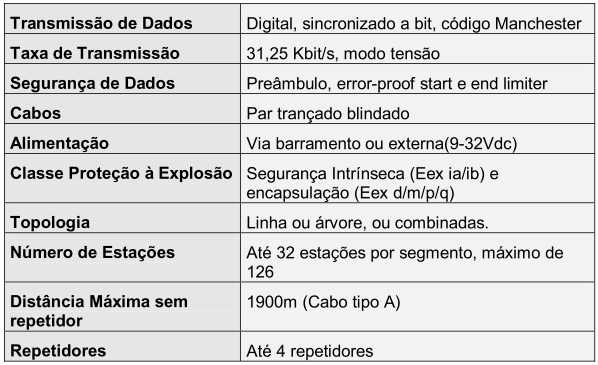
\includegraphics[scale=0.6]{figs/caracteristicas}
	\end{figure}

\end{frame}

\begin{frame}{Perfil de comunicação}{Características básicas}
	
	\begin{itemize}
		\item Velocidade;
		\item Funções de diagnóstico;
		\item Diagnóstico de estação;
		\item Diagnóstico de módulo;
		\item Diagnóstico de canal.
	\end{itemize}

\end{frame}

\begin{frame}{Perfil físico}{PROFIBUS DP}
	
	\begin{itemize}
		\item RS-485;
		\item IEC 61158-2;
		\item Fibra ótica.
	\end{itemize}

\end{frame}


\section{Aplicação}

\subsection{Exemplo}

\begin{frame}{Aplicação PROFIBUS PD}

	\begin{figure}
	\centering
	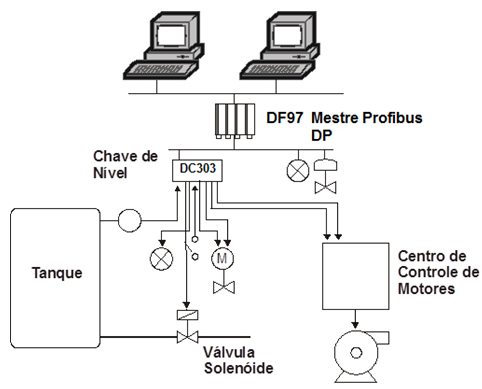
\includegraphics[scale=0.6]{figs/aplicacao}
	\end{figure}

\end{frame}

% All of the following is optional and typically not needed. 
\appendix
\section<presentation>*{\appendixname}
\subsection<presentation>*{Referências bibliográficas}

\begin{frame}[allowframebreaks]
  \frametitle<presentation>{Referências bibliográficas}
    
  \begin{thebibliography}{10}
    
  \beamertemplatebookbibitems
  % Start with overview books.

\bibitem{Z}
    {PROFIBUS
    \newblock {\em PROFIBUS}
    \newblock {Disponível em: http://www.profibus.com/technology/profibus/}
    \newblock 2015}\\
	{CASSIOLATO, C., TORRES, L. H. B., CAMARGO, P. R.
    \newblock {\em PROFIBUS - Descrição Técnica}.
    \newblock {Disponível em: http://www.smar.com/brasil/profibus}
    \newblock 2006}\\
    {RTA Automation.
    \newblock {\em PROFIBUS}
    \newblock {Disponível em: http://www.rtaautomation.com/technologies/profibus/}
    \newblock 2015}

  \beamertemplatearticlebibitems
  % Followed by interesting articles. Keep the list short. 

  \end{thebibliography}

\end{frame}

\end{document}


